All the channels were simulated in MATLAB using the 5G Toolbox. The MATLAB 5G toolbox provides a library of functions and examples for simulating the 5G NR wireless channels. This includes various physical layer models to simulate the functionality of the transmitter and receiver (e.g., modulation and encoding) as well as the different effects of the wireless channel. Figure \ref{fig:sim} shows the simulator's architecture.
\begin{figure}[H]
\centering
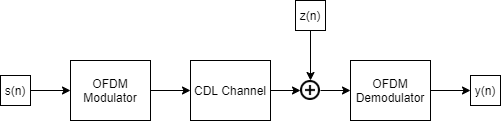
\includegraphics[width=15cm]{figures/SYSC5804-SimulationOverview.png}
\caption{Simulator Architecture}
\label{fig:sim}
\end{figure}
\noindent
The received pilots \textit{s(n)} are modulated with the 'nrOFDMModulate' modulate function. The carrier is configured to have a central frequency of 3.5GHz, a bandwidth of 90MHz, a sub-carrier spacing of 75kHz, and 32 transmit and receive antennas. These values were chosen to match those used in \cite{Li2020}. The number of antennas were varied, however most of the results were generated using 32 antennas since the resulting data sets were more manageable.  The modulated signal is passed through a 'nrCDLChannel' channel object with a custom delay profile. The CDL channel was chosen due to the configurable custom profile, it supports variable path count, gains, delays, angles, and angle spread. The simulator generates random CDL profiles for the channel model; this was used for generating diverse training data. The path count was limited to be significantly less then the number of antennas since most of the channel reconstruction algorithms required sparsity. After applying the channel effects the signal was subject to additive white Gaussian noise, $z(n)$. The noise power was a parameter of the simulation, different tests required different SNR. Finally, the signal was demodulated using 'nrOFDMDemodulate', resulting in $y(n)$, the received pilot symbols. 

The simulator aggregates the channel conditions and stores them in a CSV file along with a reference to the measurements done on the received pilots, such as the channel image discussed in the next section. The CSV has an entry for the each of the path gains, angles, and delays. The data set captures all the information needed to reconstruct the CDL channel used in the simulation. The only thing it does not capture is the noise power, antenna count and carrier details, which were typically held constant. This data set is used for training and testing the machine learning methods described in Section \ref{autodnn}.

The primary challenge faced while developing the simulator was the need for the modulation and demodulation functions. Both \cite{Li2020} and \cite{Han2019}, set all the received pilots to 1, shown mathematically, \(s(n) = 1, \forall n\) and attempted to pass these values through the channel directly. Neither paper discussed modulating the signal, so naively this step was skipped. The resulting received pilots made little sense and none of the algorithms were able to use them for channel reconstruction. For instance, the image generation held all the points against one axis, unable to move them in the angle space. After some research modulation was added to the simulator resolving these issues. 

A MATLAB script was made to test channel reconstruction from the ground truth values of the paths, it is available on GitHub titled "ChRecFromPaths.m" \cite{git}. The script simulated the wireless channel as previously described and used the received pilots without any noise as the ground truth value for the channel matrix. The equations described in \ref{sssec:chrec} were used along with the ground truth data for the paths to recreate the channel. The resulting estimated channel with a RMSE of 3.5e-05. This was considered acceptable accuracy, any error was most likely due to rounding in the floating point number math. The methods in this script would be used for channel reconstruction by the YOLO method, had the path components been properly calculated.